\section{Scroll prediction}\label{sec:scroll}

A lens over a feed is used while the feed scrolls. At the default rate the screen is captured every $125$\,ms, and the blocks that
are placed from a frame captured at $t_0$ are shown at a later display time $t$. If the content has moved by $X(t)-X(t_0)$
points in between, an unpredicted block is that far from the text it translates. At a scroll speed of $v=1000$ points per second a
frame that is only $125$\,ms old is $v\cdot0.125=125$ points off, several lines of text. The reading and the translation of a
frame take longer than that. Moving the finished blocks along with the page is therefore not an optimisation; without it the
overlay is wrong whenever the page moves.

\subsection{Model}

The application cannot ask a page how far it has scrolled, and does not need to. It sees a scroll event anywhere on the screen
(whether it scrolls what a lens reads is decided afterwards), and the system sends it with a time stamp, a signed delta $d$ in the units of the device, and a flag
that says whether the deltas are \emph{precise} (a trackpad: points, which browsers apply one to one) or \emph{lines} (a mouse wheel:
the application decides how many points a line is, and usually animates the step). Momentum scrolling needs nothing special: the
system keeps sending events that decay.

The predictor keeps the events of the last 2\,s as triples $(t_k,d_k,c_k)$ with $c_k\in\{P,L\}$ (precise, lines), positive $d$
moving the content down.\footnote{The sign convention is that of the source: a positive delta moves content down (\texttt{ScrollPredictor.swift}, the comment of \texttt{wheel}). Reading down a page moves its content up, which is a negative delta, as in the examples of Appendix~\ref{app:examples}.} Two constants describe the path from an event to the screen: a delivery latency $\lambda=16$\,ms,
and the duration $T=150$\,ms over which an application animates one line step. The fraction of event $k$ that is on screen at time $t$ is,
with $s=t-t_k-\lambda$,
\begin{equation}\label{eq:shown}
\varphi_k(t)\;=\;\begin{cases}
0 & s\le0,\\
1 & s>0,\ c_k=P,\\
1-\bigl(1-\min(1,s/T)\bigr)^3 & s>0,\ c_k=L.
\end{cases}
\end{equation}
A precise delta is a step: the content has moved all at once. A line step eases out, as in a smooth-scroll animation: it starts at
speed $3/T=20\ \mathrm{s}^{-1}$ of its total and slows to zero at $T$, so that half of it is on screen after $T(1-2^{-1/3})\approx31$\,ms, ninety percent
after $T(1-0.1^{1/3})\approx80$\,ms, and all of it after $T=150$\,ms.

\begin{figure}[t]
\centering
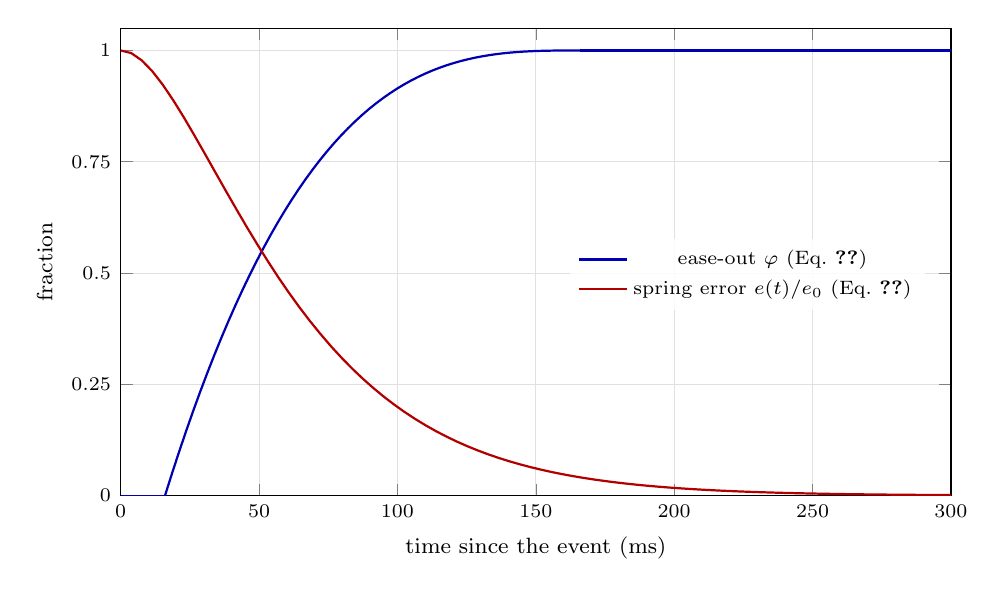
\begin{tikzpicture}
\begin{axis}[
  width=\columnwidth,height=0.62\columnwidth,
  xlabel={time since the event (ms)},ylabel={fraction},
  xmin=0,xmax=300,ymin=0,ymax=1.05,
  xtick={0,50,100,150,200,250,300},ytick={0,0.25,0.5,0.75,1},
  tick label style={font=\scriptsize},label style={font=\footnotesize},
  legend style={font=\scriptsize,at={(0.97,0.55)},anchor=north east,draw=none,fill=white,fill opacity=0.85,text opacity=1},
  grid=major,grid style={black!12},
  every axis plot/.append style={thick}
]
\addplot[blue!70!black,domain=16:166,samples=60] {1-(1-(x-16)/150)^3};
\addlegendentry{ease-out $\varphi$ (Eq.~\ref{eq:shown})}
\addplot[blue!70!black,forget plot] coordinates {(0,0) (16,0)};
\addplot[blue!70!black,forget plot,domain=166:300,samples=2] {1};
\addplot[red!70!black,domain=0:300,samples=80] {(1+0.03*x)*exp(-0.03*x)};
\addlegendentry{spring error $e(t)/e_0$ (Eq.~\ref{eq:spring})}
\end{axis}
\end{tikzpicture}

\caption{The two curves of the model, plotted from the equations, not measured: the fraction of a line step on screen
(Eq.~\ref{eq:shown} with $\lambda=16$\,ms, $T=150$\,ms) and the decay of a correction (Eq.~\ref{eq:spring}).}\label{fig:curves}
\end{figure}

\subsection{Offset between two frames}

The wheel units of kind $c$ that reached the screen between $t_0$ and $t_1$ are
\begin{equation}\label{eq:units}
U_c(t_0,t_1)\;=\;\sum_{k:\ c_k=c} d_k\,\bigl[\varphi_k(t_1)-\varphi_k(t_0)\bigr],
\end{equation}
and the content movement expected between them, in points, is
\begin{equation}\label{eq:offset}
\Delta(t_0,t_1)\;=\;\rho_P\,U_P(t_0,t_1)\;+\;\rho_L\,U_L(t_0,t_1).
\end{equation}
The ratios $\rho_c$ are points per wheel unit. $\rho_P$ starts at $1$; $\rho_L$ is unknown, and contributes $0$, until a frame has shown
how far a line goes. A display tick at time $t$ moves every block of the scroll area, which the frame $t_0$ placed, by $\Delta(t_0,t)$.

Two properties follow from the form of Eq.~(\ref{eq:units}), and the second is why the predictor needs no state beyond the
events.

\begin{proposition}[Exact tracking]\label{prop:exact}
If every event is precise, $\rho_P=1$, $\lambda=0$ and the application moves the content by exactly $d_k$ at $t_k$, then
$\Delta(t_0,t_1)=\sum_{t_0\le t_k<t_1}d_k=X(t_1)-X(t_0)$.
\end{proposition}

\begin{proposition}[Re-basing]\label{prop:rebase}
For $t_0\le t_1\le t$ and fixed ratios, $\Delta(t_0,t)=\Delta(t_0,t_1)+\Delta(t_1,t)$.
\end{proposition}

\noindent Both are one line: $\varphi_k(t_1)-\varphi_k(t_0)$ is a difference, and the differences telescope. The first is a unit
test (ten events of $-4$ points, the frame placed in the middle of them: five are left and $\Delta=-20$). The second means that when
the next frame, captured at $t_1$, contains the movement up to $t_1$, the display only has to add $\Delta(t_1,t)$: nothing is
counted twice and nothing is lost at the frame boundary. It also means that a wrong ratio produces an error that the next frame
can measure.

\subsection{What the frame confirms}

Each captured frame is compared with the previous one. A band of columns that changed is matched against the previous frame by the
mean absolute difference of its gray pixels over the rows that overlap after a shift $d$,
\begin{equation*}
\mathrm{err}(d)\;=\;\frac1{|\Omega_d|}\sum_{(x,y)\in\Omega_d}\bigl|a(x,y)-b(x,y+d)\bigr| ,
\end{equation*}
sampling every other column. The shift is searched over whole pixels, at most a quarter of the band's height, and then refined by $\pm0.5$ and $\pm0.25$ with the two nearest
rows of $b$ blended, so smooth scrolling is resolved to a quarter of a pixel of the downsampled image. It is accepted only when
$|d|\ge0.25$, $\mathrm{err}(d)<0.6\,\mathrm{err}(0)$ and $\mathrm{err}(d)<8$. A band too plain to be matched on its own takes its
neighbour's shift if that explains it better than no move; neighbouring bands whose shifts differ by at most $0.5$ form one
\emph{region}, and a region shorter than three tiles is something moving in place, not a scroll. Pages keep fixed parts (headers,
sidebars, an input box) beside the part that scrolls, which is why the match is made per column band and not for the whole frame.

A region that holds the pointer yields a \emph{report}: the shift $\sigma$ in points (positive = down) and the capture times $t_0,t_1$ of
the two frames. The predictor learns from it. Let $u_P=U_P(t_0,t_1)$ and $u_L=U_L(t_0,t_1)$. The report is used only if exactly one of
$|u_P|,|u_L|$ is at least one unit (it cannot tell two ratios apart from one shift). With $c$ the kind that has units, the sample is
$\hat\rho=\sigma/u_c$ and
\begin{equation}\label{eq:confirm}
\rho_c\;\leftarrow\;\begin{cases}
\hat\rho & \rho_c\ \text{unknown},\\
\rho_c+0.3\,(\hat\rho-\rho_c) & 0.33<\hat\rho/\rho_c<3,\\
\rho_c & \text{otherwise,}
\end{cases}
\end{equation}
where the first case also needs $\hat\rho$ finite and nonzero. The gate around $\rho_c$ ignores what says nothing: a stop at the end of the page (events but no movement), or a scroll by other means (keys, scripts). In the
unit test, fifty precise units with a ratio of $1$ meet a frame that shows $-60$ points: $\hat\rho=1.2$, the ratio becomes $1+0.3\cdot0.2=1.06$ and the
next offset for the same events is $-53$. Without noise, the error of $\rho_c$ shrinks by the factor $0.7$ with every accepted
report, to $17\%$ after five and $2.8\%$ after ten. The ratio belongs to the application and page under the pointer, so it is forgotten when
a new gesture starts over a different window.

The prediction is used only while events keep coming: the overlay asks for $\Delta$ only if the last event is less than
one second old and a scroll area is known (first guessed as the lens's part of the window under the pointer, and
corrected by the first frame that moves).

\subsection{Correcting the display}

When the next frame arrives, the blocks it has moved are where the content is, and the blocks the display showed were where the
prediction put them. The difference $e$ is an error of the prediction, and a jump of $e$ would show as a jolt. If $|e|<80$ points the layer
is given an additive spring animation from $e$ to $0$ with mass $m=1$ and stiffness $k=900$, and the damping is set to the critical value
$c=2\sqrt{km}=60$. With $\omega_0=\sqrt{k/m}=30$ rad/s and zero initial velocity (the default of the animation, which the code does not
set), the remaining error is
\begin{equation}\label{eq:spring}
e(t)\;=\;e_0\,(1+\omega_0t)\,e^{-\omega_0t},
\end{equation}
which has no overshoot. It is down to $5\%$ of $e_0$ after $158$\,ms and to $1\%$ after $221$\,ms. A correction that is still easing in when
the next one arrives carries on from where the block is seen, not from where it was going. Ending a prediction, when the events stop, is a correction too:
whatever the frames have not confirmed eases away.

\begin{algorithm}[t]
\caption{Predict and correct, per lens.}\label{alg:predict}
\begin{algorithmic}[1]
\Procedure{OnWheel}{$e$}
  \If{$e$ starts a gesture over another window} \State reset $\rho_P\gets1$, $\rho_L\gets\bot$, forget the events \EndIf
  \State append $(t_e,d_e,c_e)$, drop events older than 2\,s
  \State $t_\ell\gets t_e$
\EndProcedure
\Procedure{OnTick}{$t$}\Comment{every display frame}
  \If{$t-t_\ell<1$\,s \textbf{and} the scroll area is known} \State $\Delta\gets\rho_PU_P(t_f,t)+\rho_LU_L(t_f,t)$
  \Else\ \State $\Delta\gets0$ \EndIf
  \ForAll{block $b$ in the scroll area}
    \State $e\gets\mathrm{shown}_b-(y_b+\Delta)$; \ $\mathrm{shown}_b\gets y_b+\Delta$
    \If{correcting \textbf{and} $0<|e|<80$} \State add a critically damped spring \EndIf
  \EndFor
\EndProcedure
\Procedure{OnFrame}{frame at $t_1$, previous frame at $t_0$}
  \ForAll{scroll region $r$ with shift $\sigma$}
    \State move the blocks in $r$ by $\sigma$
    \If{$r$ holds the pointer} \State confirm$(\sigma,t_0,t_1)$ by Eq.~(\ref{eq:confirm}) \EndIf
  \EndFor
  \State $t_f\gets t_1$; \ \Call{OnTick}{now} with correcting
\EndProcedure
\end{algorithmic}
\end{algorithm}

\subsection{Drift}

The quantity that matters is how far a shown translation is from the text it translates. The self-test measures it. For each block it records, when the
block is first seen, its position on the \emph{page}: the on-screen position plus the scroll offset for blocks inside the scrolling rectangle. At
every captured step $f$ it takes the largest displacement of any shown block from that anchor,
\begin{equation}\label{eq:drift}
D_f\;=\;\max_{b\in B_f}\ \bigl\|p_b(f)-p_b(0)\bigr\|_2,
\end{equation}
and prints $D_f$ per frame and, at the end, the mean of $D_f$, the maximum, and the number of frames with $D_f>2$ points. A block that is re-laid out is
anchored again. With exact prediction every block stays on its text and $D_f=0$ (Proposition~\ref{prop:exact}); without it, $D_f$ is the distance the page has moved since the frame the block was placed from. In the
self-test the application is simulated with $\lambda=0$ and wheel deltas equal to the true scroll, which is the best case for the predictor: drift there isolates what the pipeline adds, and a real application
adds its own animation and the error of $\rho$ on top.

Listing~\ref{lst:scroll} is the predictor. It has no dependency on the system: it takes times as numbers, which is how the unit tests drive it.

\begin{listing*}[t]
\lstinputlisting[firstnumber=31]{listings/ScrollPredictor_core.swift}
\caption{The core of \code{ScrollPredictor}, \texttt{Core/Sources/MwoyeoCore/ScrollPredictor.swift}, lines 31--68 (\code{offset},
\code{confirm}, \code{reset}, \code{units}, \code{shown}), as it is in the repository. \code{shown} is Eq.~(\ref{eq:shown}),
\code{units} Eq.~(\ref{eq:units}), \code{offset} Eq.~(\ref{eq:offset}) and \code{confirm} Eq.~(\ref{eq:confirm}).}\label{lst:scroll}
\end{listing*}
